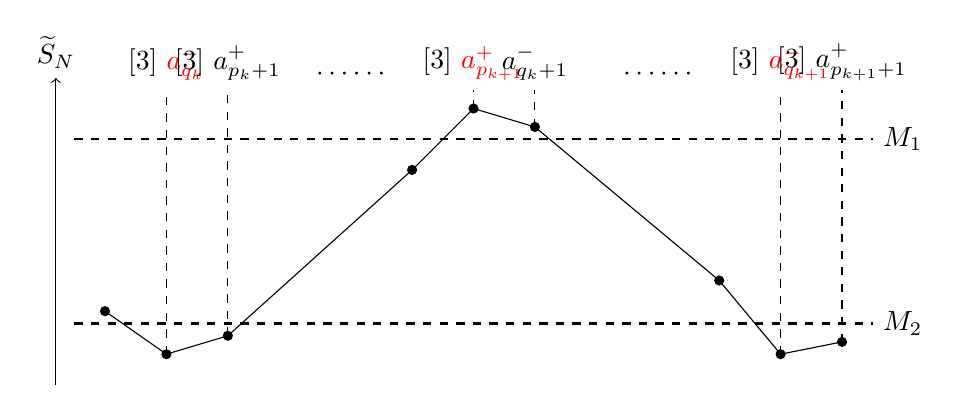
\begin{tikzpicture}[
scale=0.78,
]

\draw[->] (-0.8, -2.5) -- (-0.8, 2.5) node[anchor=south] {$\widetilde{S}_N$};
\draw[dashed, thick] (-0.5,  1.5) -- (12.5,  1.5) node[right] {$M_1$};
\draw[dashed, thick] (-0.5, -1.5) -- (12.5, -1.5) node[right] {$M_2$};

% Same x-coordinates as riemann-series-thm.tex: 0,1,2,5,6,7,10,11,12
% Peaks exceed +M, valleys drop below -M; amplitudes do not shrink (oscillating divergence)
\draw[thin]
    (0, -1.3) node[fill,circle,inner sep=1.3pt]{}
    \foreach \x/\y in {1/-2.0, 2/-1.7, 5/1.0, 6/2.0, 7/1.7, 10/-0.8, 11/-2.0, 12/-1.8} {
        -- (\x,\y) node[fill,circle,inner sep=1.3pt]{}
    };

% All dashed lines go from current dot's y up to label area (no amplitude arrow)
\draw[dashed, thin] (1, -2.0) -- (1,  2.3) node[anchor=south] {\smaller[3] \color{red} $a_{q_k}^-$};
\draw[dashed, thin] (2, -1.7) -- (2,  2.3) node[anchor=south] {\smaller[3] $a_{p_k+1}^+$};
\draw[dashed, thin] (6,  2.0) -- (6,  2.3) node[anchor=south] {\smaller[3] \color{red} $a_{p_{k+1}}^+$};
\draw[dashed, thin] (7,  1.7) -- (7,  2.3) node[above]        {\smaller $a_{q_k+1}^-$};
\draw[dashed, thin] (11,-2.0) -- (11, 2.3) node[anchor=south] {\smaller[3] \color{red} $a_{q_{k+1}}^-$};
\draw[dashed, thin] (12,-1.8) -- (12, 2.3) node[anchor=south] {\smaller[3] $a_{p_{k+1}+1}^+$};

\node[anchor=south] at (4, 2.3) {$\cdots\cdots$};
\node[anchor=south] at (9, 2.3) {$\cdots\cdots$};

\end{tikzpicture}
